\documentclass{article}
\usepackage[a4paper, portrait, margin=1in]{geometry}
\usepackage{graphicx}
\usepackage{array}
\usepackage{listings}
\usepackage{xcolor}
\usepackage[utf8]{inputenc}
\usepackage{blindtext}
\usepackage[export]{adjustbox}

\definecolor{codegreen}{rgb}{0,0.6,0}
\definecolor{codegray}{rgb}{0.5,0.5,0.5}
\definecolor{codepurple}{rgb}{0.58,0,0.82}
\definecolor{backcolour}{rgb}{0.95,0.95,0.92}

\lstdefinestyle{mystyle}{
    backgroundcolor=\color{backcolour},   
    commentstyle=\color{codegreen},
    keywordstyle=\color{magenta},
    numberstyle=\tiny\color{codegray},
    stringstyle=\color{codepurple},
    breakatwhitespace=false,         
    breaklines=true,                 
    captionpos=b,                    
    keepspaces=true,                 
    numbers=left,                    
    numbersep=5pt,                  
    showspaces=false,                
    showstringspaces=false,
    showtabs=false,                  
    tabsize=4
}
 
 

\begin{document}

\title{Student Id: 9910821}
\date{}

\maketitle

\section*{Task 1}
Formula for the value $h$ given by
\begin{equation}
h = \frac{ X_r-f(r,t,T)}{\sqrt{v^2(t,T)}}.
\end{equation}

\section*{Task 2}
Value of the put option $V(r,t,T)$ is 
\begin{equation}
V(r,t,T) = 0.549
\end{equation}
with parameters $r=0.052$, $t=0$, $T=2$, $X_r=0.06$, $\kappa=0.0944$, $\theta=0.0616$, $\sigma=0.0317$.

\section*{Task 3}
\begin{figure}[h]
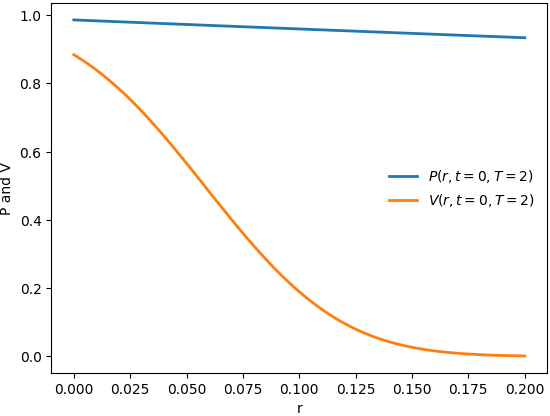
\includegraphics[width=0.7\textwidth,center]{plot.png}
\caption{A plot of the functions of bond price $P$ and the option price $V$ for different interest rates $r$.}
\end{figure}


\section*{Program listings}
\lstset{style=mystyle}
\subsection*{Pricing Generator Listing}
\lstinputlisting[language=C++]{../assignment_2.cpp}
\subsection*{Graphing Package Listing}
\lstinputlisting[language=Python]{../assignment_2.py}
\end{document}